%        File: arfc-beamer.tex
%     Created: Sun May 5 10:00 PM 2013 C
%


%\documentclass[11pt,handout]{beamer}
\documentclass[9pt]{beamer}
\usetheme[white]{Illinois}
%\title[short title]{long title}
\title{Simulation of Molten Salt Reactors with Moltres}
%\subtitle[short subtitle]{long subtitle}
%\subtitle[Short SubTitle]{Mostly Kittens}
%\author[short name]{long name}
\author[Andrei Rykhlevskii]{Andrei Rykhlevskii\inst{1}, Alexander Lindsay\inst{2}, Kathryn Huff\inst{1}\\Advanced Reactors and Fuel Cycles Group}
%\date[short date]{long date}
\date[02.26.2019]{Feb 26, 2019}
%\institution[short name]{long name}
\institute[UIUC]{\inst{1} University of Illinois at Urbana-Champaign \and \inst{2} Idaho National Laboratory}


\usepackage{lmodern}

%\usepackage{bbding}
\usepackage{tikz}
\usepackage{amsfonts}
\usepackage{amsmath}
\usepackage{caption}  % allows center figures caption
\usepackage{xspace}
\usepackage{notoccite}
\usepackage{graphicx}
\usepackage{animate}
\usepackage{subfigure}
\usepackage{media9}
\usepackage{booktabs} % nice rules for tables
\usepackage{microtype} % if using PDF
\usepackage{bigints}
%\usepackage{minted}
\usepackage{xcolor}
\usepackage{soul}
\newcommand{\hlc}[2][yellow]{{%
    \colorlet{foo}{#1}%
    \sethlcolor{foo}\hl{#2}}%
}
\newcommand{\units}[1] {\:\text{#1}}%
\newcommand{\SN}{S$_N$}%{S$_\text{N}$}%{$S_N$}%
\DeclareMathOperator{\erf}{erf}
%I need some complimentary error funcitons... 
\DeclareMathOperator{\erfc}{erfc}
%page numbers
\setbeamertemplate{footline}[page number]
\setbeamertemplate{caption}[numbered]
%Those icons in the references are terrible looking
\setbeamertemplate{bibliography item}[text]

%%%% Acronym support

\usepackage[acronym,toc]{glossaries}
%\newacronym{<++>}{<++>}{<++>}
\newacronym[longplural={metric tons of heavy metal}]{MTHM}{MTHM}{metric ton of heavy metal}
\newacronym{ABM}{ABM}{agent-based modeling}
\newacronym{ACDIS}{ACDIS}{Program in Arms Control \& Domestic and International Security}
\newacronym{AHTR}{AHTR}{Advanced High Temperature Reactor}
\newacronym{ANDRA}{ANDRA}{Agence Nationale pour la gestion des D\'echets RAdioactifs, the French National Agency for Radioactive Waste Management}
\newacronym{ANL}{ANL}{Argonne National Laboratory}
\newacronym{ANS}{ANS}{American Nuclear Society}
\newacronym{AOA}{AOA}{Axial Offset Anomaly}
\newacronym{API}{API}{application programming interface}
\newacronym{ARE}{ARE}{Aircraft Reactor Experiment}
\newacronym{ARFC}{ARFC}{Advanced Reactors and Fuel Cycles}
\newacronym{ASME}{ASME}{American Society of Mechanical Engineers}
\newacronym{ATWS}{ATWS}{Anticipated Transient Without Scram}
\newacronym{BOL}{BOL}{Beginning of Life}
\newacronym{BDBE}{BDBE}{Beyond Design Basis Event}
\newacronym{BIDS}{BIDS}{Berkeley Institute for Data Science}
\newacronym{BWR}{BWR}{Boiling Water Reactor}
\newacronym{CAFCA}{CAFCA}{ Code for Advanced Fuel Cycles Assessment }
\newacronym{CDTN}{CDTN}{Centro de Desenvolvimento da Tecnologia Nuclear}
\newacronym{CFD}{CFD}{Computational Fluid Dynamics}
\newacronym{CEA}{CEA}{Commissariat \`a l'\'Energie Atomique et aux \'Energies Alternatives}
\newacronym{CI}{CI}{continuous integration}
\newacronym{CNEN}{CNEN}{Comiss\~{a}o Nacional de Energia Nuclear}
\newacronym{CNERG}{CNERG}{Computational Nuclear Engineering Research Group}
\newacronym{COSI}{COSI}{Commelini-Sicard}
\newacronym{COTS}{COTS}{commercial, off-the-shelf}
\newacronym{CSNF}{CSNF}{commercial spent nuclear fuel}
\newacronym{CTAH}{CTAHs}{Coiled Tube Air Heaters}
\newacronym{CUBIT}{CUBIT}{CUBIT Geometry and Mesh Generation Toolkit}
\newacronym{CURIE}{CURIE}{Centralized Used Fuel Resource for Information Exchange}
\newacronym{CR}{CR}{conversion ratio}
\newacronym{DAG}{DAG}{directed acyclic graph}
\newacronym{DANESS}{DANESS}{Dynamic Analysis of Nuclear Energy System Strategies}
\newacronym{DBE}{DBE}{Design Basis Event}
\newacronym{DESAE}{DESAE}{Dynamic Analysis of Nuclear Energy Systems Strategies}
\newacronym{DHS}{DHS}{Department of Homeland Security}
\newacronym{DOE}{DOE}{Department of Energy}
\newacronym{DRACS}{DRACS}{Direct Reactor Auxiliary Cooling System}
\newacronym{DRE}{DRE}{dynamic resource exchange}
\newacronym{DSNF}{DSNF}{DOE spent nuclear fuel}
\newacronym{DYMOND}{DYMOND}{Dynamic Model of Nuclear Development }
\newacronym{EBS}{EBS}{Engineered Barrier System}
\newacronym{EDF}{EDF}{Électricité de France}
\newacronym{EDZ}{EDZ}{Excavation Disturbed Zone}
\newacronym{EOL}{EOL}{End of Life}
\newacronym{EIA}{EIA}{U.S. Energy Information Administration}
\newacronym{EPA}{EPA}{Environmental Protection Agency}
\newacronym{EPR}{EPR}{European Pressurized Reactors}
\newacronym{EP}{EP}{Engineering Physics}
\newacronym{EU}{EU}{European Union}
\newacronym{FCO}{FCO}{Fuel Cycle Options}
\newacronym{FCT}{FCT}{Fuel Cycle Technology}
\newacronym{FEHM}{FEHM}{Finite Element Heat and Mass Transfer}
\newacronym{FEPs}{FEPs}{Features, Events, and Processes}
\newacronym{FHR}{FHR}{Fluoride-Salt-Cooled High-Temperature Reactor}
\newacronym{FLiBe}{FLiBe}{Fluoride-Lithium-Beryllium}
\newacronym{FP}{FP}{Fission Product}
\newacronym{FTC}{FTC}{fuel temperature coefficient}
\newacronym{GDSE}{GDSE}{Generic Disposal System Environment}
\newacronym{GDSM}{GDSM}{Generic Disposal System Model}
\newacronym{GENIUSv1}{GENIUSv1}{Global Evaluation of Nuclear Infrastructure Utilization Scenarios, Version 1}
\newacronym{GENIUSv2}{GENIUSv2}{Global Evaluation of Nuclear Infrastructure Utilization Scenarios, Version 2}
\newacronym{GENIUS}{GENIUS}{Global Evaluation of Nuclear Infrastructure Utilization Scenarios}
\newacronym{GPAM}{GPAM}{Generic Performance Assessment Model}
\newacronym{GRSAC}{GRSAC}{Graphite Reactor Severe Accident Code}
\newacronym{GUI}{GUI}{graphical user interface}
\newacronym{HFP}{HFP}{hot full power}
\newacronym{HLW}{HLW}{high level waste}
\newacronym{HPC}{HPC}{high-performance computing}
\newacronym{HTC}{HTC}{high-throughput computing}
\newacronym{HTGR}{HTGR}{High Temperature Gas-Cooled Reactor}
\newacronym{HZP}{HZP}{hot zero power}
\newacronym{IAEA}{IAEA}{International Atomic Energy Agency}
\newacronym{IEMA}{IEMA}{Illinois Emergency Mangament Agency}
\newacronym{IHLRWM}{IHLRWM}{International High Level Radioactive Waste Management}
\newacronym{INL}{INL}{Idaho National Laboratory}
\newacronym{IPRR1}{IRP-R1}{Instituto de Pesquisas Radioativas Reator 1}
\newacronym{IRP}{IRP}{Integrated Research Project}
\newacronym{ISFSI}{ISFSI}{Independent Spent Fuel Storage Installation}
\newacronym{ISRG}{ISRG}{Independent Student Research Group}
\newacronym{JFNK}{JFNK}{Jacobian-Free Newton Krylov}
\newacronym{LANL}{LANL}{Los Alamos National Laboratory}
\newacronym{LBNL}{LBNL}{Lawrence Berkeley National Laboratory}
\newacronym{LCOE}{LCOE}{levelized cost of electricity}
\newacronym{LEU}{LEU}{low-enriched uranium}
\newacronym{LDRD}{LDRD}{laboratory directed research and development}
\newacronym{LFR}{LFR}{Lead-Cooled Fast Reactor}
\newacronym{LLNL}{LLNL}{Lawrence Livermore National Laboratory}
\newacronym{LMFBR}{LMFBR}{Liquid Metal Fast Breeder Reactor}
\newacronym{LOFC}{LOFC}{Loss of Forced Cooling}
\newacronym{LOHS}{LOHS}{Loss of Heat Sink}
\newacronym{LOLA}{LOLA}{Loss of Large Area}
\newacronym{LP}{LP}{linear program}
\newacronym{LWR}{LWR}{Light Water Reactor}
\newacronym{MAGNOX}{MAGNOX}{Magnesium Alloy Graphie Moderated Gas Cooled Uranium Oxide Reactor}
\newacronym{MA}{MA}{minor actinide}
\newacronym{MCNP}{MCNP}{Monte Carlo N-Particle code}
\newacronym{MCFR}{MCSFR}{Molten Chloride Fast Reactor}
\newacronym{MILP}{MILP}{mixed-integer linear program}
\newacronym{MIT}{MIT}{the Massachusetts Institute of Technology}
\newacronym{MOAB}{MOAB}{Mesh-Oriented datABase}
\newacronym{MOOSE}{MOOSE}{Multiphysics Object-Oriented Simulation Environment}
\newacronym{MOSART}{MOSART}{Molten Salt Actinide Recycler and Transmuter}
\newacronym{MOX}{MOX}{mixed oxide}
\newacronym{MPI}{MPI}{Message Passing Interface}
\newacronym{MSBR}{MSBR}{Molten Salt Breeder Reactor}
\newacronym{MSFR}{MSFR}{Molten Salt Fast Reactor}
\newacronym{MSRE}{MSRE}{Molten Salt Reactor Experiment}
\newacronym{MSR}{MSR}{Molten Salt Reactor}
\newacronym{MTC}{MTC}{moderator temperature coefficient}
\newacronym{NAGRA}{NAGRA}{National Cooperative for the Disposal of Radioactive Waste}
\newacronym{NEAMS}{NEAMS}{Nuclear Engineering Advanced Modeling and Simulation}
\newacronym{NEUP}{NEUP}{Nuclear Energy University Programs}
\newacronym{NFCSim}{NFCSim}{Nuclear Fuel Cycle Simulator}
\newacronym{NGNP}{NGNP}{Next Generation Nuclear Plant}
\newacronym{NMWPC}{NMWPC}{Nuclear MW Per Capita}
\newacronym{NNSA}{NNSA}{National Nuclear Security Administration}
\newacronym{NPP}{NPP}{Nuclear Power Plant}
\newacronym{NPRE}{NPRE}{Department of Nuclear, Plasma, and Radiological Engineering}
\newacronym{NQA1}{NQA-1}{Nuclear Quality Assurance - 1}
\newacronym{NRC}{NRC}{Nuclear Regulatory Commission}
\newacronym{NSF}{NSF}{National Science Foundation}
\newacronym{NSSC}{NSSC}{Nuclear Science and Security Consortium}
\newacronym{NUWASTE}{NUWASTE}{Nuclear Waste Assessment System for Technical Evaluation}
\newacronym{NWF}{NWF}{Nuclear Waste Fund}
\newacronym{NWTRB}{NWTRB}{Nuclear Waste Technical Review Board}
\newacronym{OCRWM}{OCRWM}{Office of Civilian Radioactive Waste Management}
\newacronym{OOP}{OOP}{Object-Oriented Programming}
\newacronym{ORION}{ORION}{ORION}
\newacronym{ORNL}{ORNL}{Oak Ridge National Laboratory}
\newacronym{PARCS}{PARCS}{Purdue Advanced Reactor Core Simulator}
\newacronym{PBAHTR}{PB-AHTR}{Pebble Bed Advanced High Temperature Reactor}
\newacronym{PBFHR}{PB-FHR}{Pebble-Bed Fluoride-Salt-Cooled High-Temperature Reactor}
\newacronym{PEI}{PEI}{Peak Environmental Impact}
\newacronym{PH}{PRONGHORN}{PRONGHORN}
\newacronym{PRIS}{PRIS}{Power Reactor Information System}
\newacronym{PRKE}{PRKE}{Point Reactor Kinetics Equations}
\newacronym{PSPG}{PSPG}{Pressure-Stabilizing/Petrov-Galerkin}
\newacronym{PWAR}{PWAR}{Pratt and Whitney Aircraft Reactor}
\newacronym{PWR}{PWR}{Pressurized Water Reactor}
\newacronym{PyNE}{PyNE}{Python toolkit for Nuclear Engineering}
\newacronym{PyRK}{PyRK}{Python for Reactor Kinetics}
\newacronym{QA}{QA}{quality assurance}
\newacronym{RDD}{RD\&D}{Research Development and Demonstration}
\newacronym{RD}{R\&D}{Research and Development}
\newacronym{REE}{REE}{rare earth element}
\newacronym{RELAP}{RELAP}{Reactor Excursion and Leak Analysis Program}
\newacronym{RIA}{RIA}{Reactivity Insertion Accident}
\newacronym{RIF}{RIF}{Region-Institution-Facility}
\newacronym{SFR}{SFR}{Sodium-Cooled Fast Reactor}
\newacronym{SINDAG}{SINDA{\textbackslash}G}{Systems Improved Numerical Differencing Analyzer $\backslash$ Gaski}
\newacronym{SKB}{SKB}{Svensk K\"{a}rnbr\"{a}nslehantering AB}
\newacronym{SNF}{SNF}{spent nuclear fuel}
\newacronym{SNL}{SNL}{Sandia National Laboratory}
\newacronym{STC}{STC}{specific temperature change}
\newacronym{SUPG}{SUPG}{Streamline-Upwind/Petrov-Galerkin}
\newacronym{SWF}{SWF}{Separations and Waste Forms}
\newacronym{SWU}{SWU}{Separative Work Unit}
\newacronym{TAP}{TAP}{Transatomic Power}
\newacronym{TRIGA}{TRIGA}{Training Research Isotope General Atomic}
\newacronym{TRISO}{TRISO}{Tristructural Isotropic}
\newacronym{TSM}{TSM}{Total System Model}
\newacronym{TSPA}{TSPA}{Total System Performance Assessment for the Yucca Mountain License Application}
\newacronym{ThOX}{ThOX}{thorium oxide}
\newacronym{UFD}{UFD}{Used Fuel Disposition}
\newacronym{UML}{UML}{Unified Modeling Language}
\newacronym{UOX}{UOX}{uranium oxide}
\newacronym{UQ}{UQ}{uncertainty quantification}
\newacronym{US}{US}{United States}
\newacronym{UW}{UW}{University of Wisconsin}
\newacronym{VISION}{VISION}{the Verifiable Fuel Cycle Simulation Model}
\newacronym{VVER}{VVER}{Voda-Vodyanoi Energetichesky Reaktor (Russian Pressurized Water Reactor)}
\newacronym{VV}{V\&V}{verification and validation}
\newacronym{WIPP}{WIPP}{Waste Isolation Pilot Plant}
\newacronym{YMR}{YMR}{Yucca Mountain Repository Site}


\makeglossaries

%try to get rid of header on title page\dots
\makeatletter
    \newenvironment{withoutheadline}{
        \setbeamertemplate{headline}[default]
        \def\beamer@entrycode{\vspace*{-\headheight}}
    }{}
\makeatother

\begin{document}
%%%%%%%%%%%%%%%%%%%%%%%%%%%%%%%%%%%%%%%%%%%%%%%%%%%%%%%%%%%%%
%% From uw-beamer Here's a handy bit of code to place at 
%% the beginning of your presentation (after \begin{document}):
\newcommand*{\alphabet}{ABCDEFGHIJKLMNOPQRSTUVWXYZabcdefghijklmnopqrstuvwxyz}
\newlength{\highlightheight}
\newlength{\highlightdepth}
\newlength{\highlightmargin}
\setlength{\highlightmargin}{2pt}
\settoheight{\highlightheight}{\alphabet}
\settodepth{\highlightdepth}{\alphabet}
\addtolength{\highlightheight}{\highlightmargin}
\addtolength{\highlightdepth}{\highlightmargin}
\addtolength{\highlightheight}{\highlightdepth}
\newcommand*{\Highlight}{\rlap{\textcolor{HighlightBackground}{\rule[-\highlightdepth]{\linewidth}{\highlightheight}}}}
%%%%%%%%%%%%%%%%%%%%%%%%%%%%%%%%%%%%%%%%%%%%%%%%%%%%%%%%%%%%%
%%--------------------------------%%
\begin{withoutheadline}
\frame{
  \titlepage
}
\end{withoutheadline}

%%--------------------------------%%
\AtBeginSection[]{
\begin{frame}
  \frametitle{Outline}
  \tableofcontents[currentsection]
\end{frame}
}

\section{Introduction}
\subsection{About ARFC}
\begin{frame}
  \frametitle{Advanced Reactors and Fuel Cycles group (PI: Kathryn Huff)}
               \begin{figure}[t]
                \vspace*{-0.25in}
                \hspace*{-0.35in}
                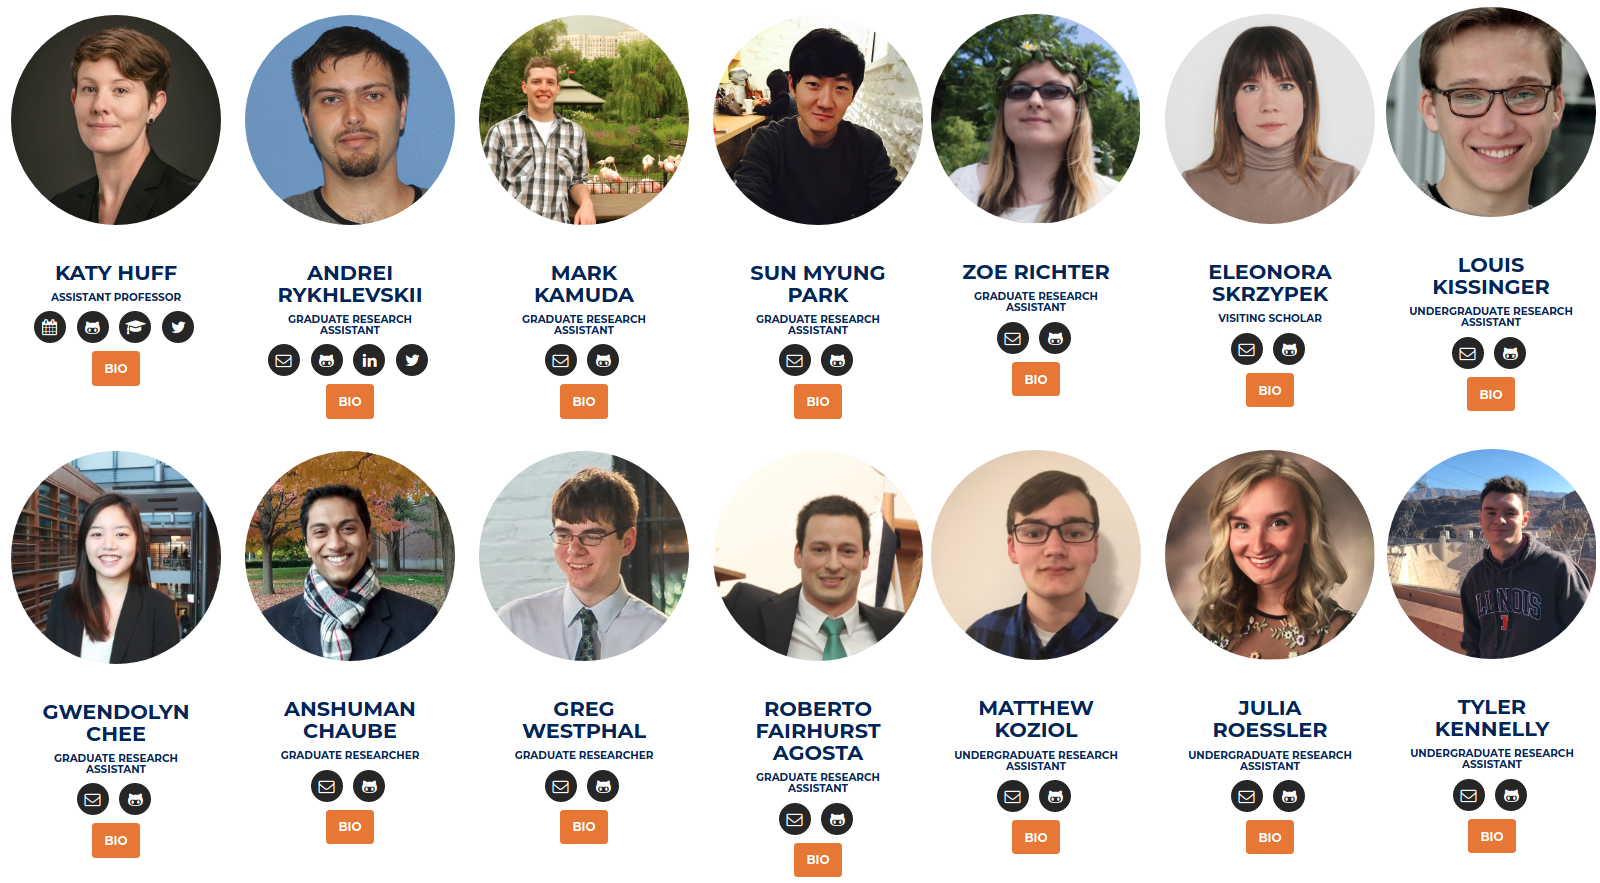
\includegraphics[height=0.63\textwidth]{./images/arfc1.png}
                \caption{Current Advanced Reactors and Fuel Cycles Group researchers.}
               \end{figure}            
\end{frame}

\begin{frame}
  \frametitle{Advanced Reactors and Fuel Cycles group (PI: Kathryn Huff)}
               \begin{figure}[t]
                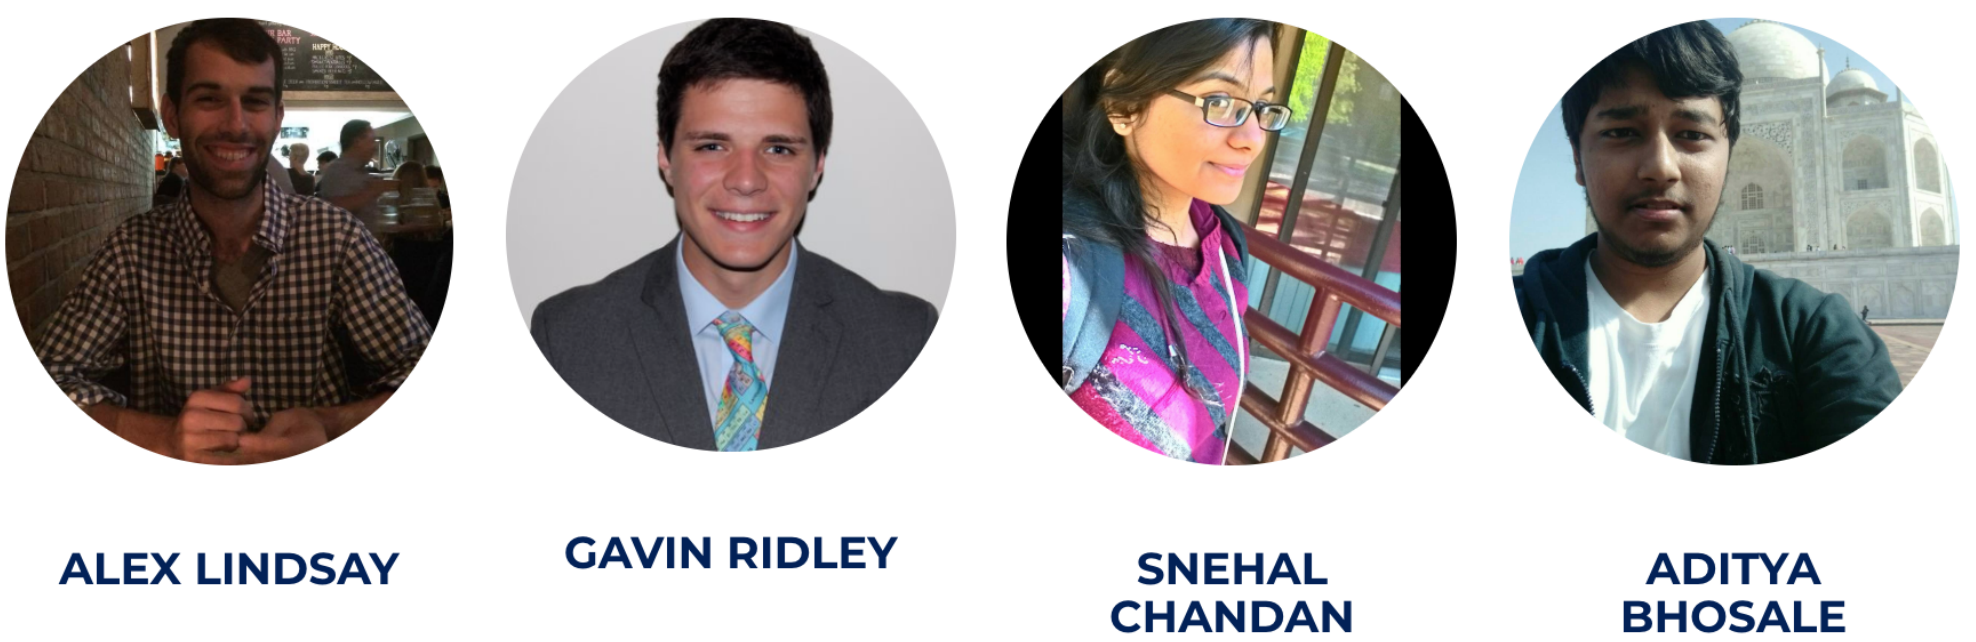
\includegraphics[height=0.33\textwidth]{./images/arfc_past.png}
                \caption{Past ARFC Group members who contributed to this work.}
               \end{figure}            
\end{frame}


\begin{frame}
  \frametitle{Insights at Disparate Scales}
               \begin{figure}[t]
                \vspace*{-0.1in}
			\hspace*{-0.35in}
                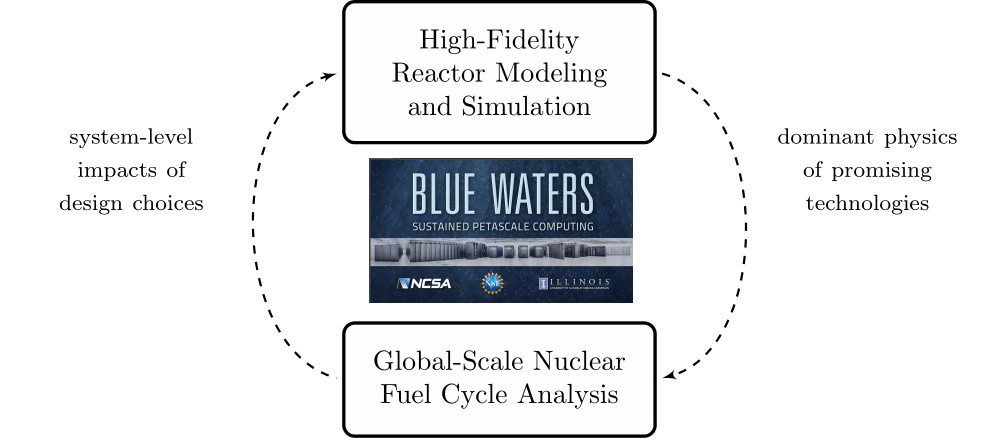
\includegraphics[height=0.5\textwidth]{./images/synergy.png}
               \end{figure}            
\end{frame}

\subsection{Molten salt reactors}
\begin{frame}
  \frametitle{Molten Salt Reactor Types}
                  \vspace*{-0.1in}
              \begin{block}{Stationary Fuel}
               \begin{enumerate}
                \item Graphite block with TRISO fuel, clean salt works as coolant (e.g. TMSR-SF1, FHR-DR)
                \item Plate Fuel: hexagonal fuel assembly is similar in shape to a typical sodium-cooled reactor
                        % Not sure what FIRM is.
                %\item Fuel Inside Radial Moderator (FIRM)
                        % While it doesn't leave the reactor, doesn't 
                        % the fuel in the moltex reactor move up and down?
                        % If the fluid is free to naturally circulate inside 
                        % the rod, it likely happens on 
                        % timescales that I do not think we can ignore from a 
                        % kinetics perspective. 
                %\item Liquid fuel salt inside fuel rods cooled by clean salt (e.g. Moltex Stable Salt Reactor)
               \end{enumerate}
               \end{block}
               
               \begin{block}{Mobile Fuel}
               \begin{enumerate}
                \item Mobile solid fuel elements (e.g. pebbles) cooled by clean salt (e.g. PB-FHR)
                \item Non-circulating liquid fuel salt (e.g. TerraPower MCFR) 
                \item \textbf{Circulating fuel salt} which also works as coolant (e.g. \gls{MSRE}, \gls{MSBR}, TAP MSR)
               \end{enumerate}
               \end{block}
\end{frame}

\begin{frame}
  \frametitle{Stationary and Mobile Solid fuel}
        \vspace*{-0.1in}
               \begin{figure}[t]
			\hspace*{-0.35in}
                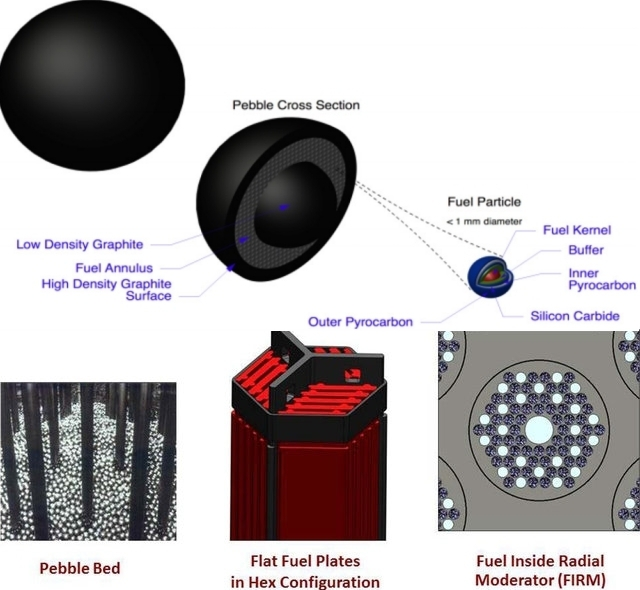
\includegraphics[height=0.63\textwidth]{./images/solid_fuel.jpg}
                \caption{TRISO fuel particle (top) and FHR fuel designs (bottom). Source \cite{forsberg_basis_2016-1}.}
             \end{figure}   
  
\end{frame}

\begin{frame}
  \frametitle{Mobile, Non-Circulating, Liquid Fuel}
               \begin{figure}[t]
                \vspace*{-0.1in}
			\hspace*{-0.35in}
                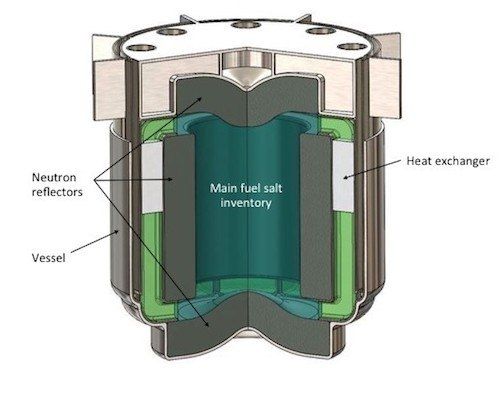
\includegraphics[height=0.6\textwidth]{./images/mcfr-crossection.jpg}
                \caption{The TerraPower MCFR is an example of reactor design with \textbf{liquid, mobile, non-circulating} chloride salt fuel. Source \cite{doene_southern_2018}.}
             \end{figure}   
  
\end{frame}

\begin{frame}
  \frametitle{Mobile, Circulating, Liquid Fuel}
               \begin{figure}[t]
                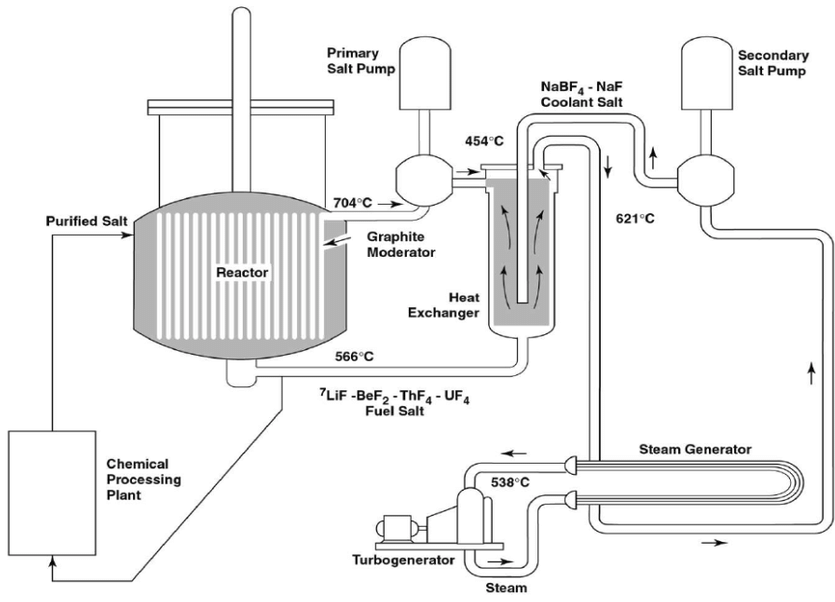
\includegraphics[height=0.58\textwidth]{./images/msbr_scheme.png}
                \caption{The \gls{MSBR} is an example of reactor design with \textbf{liquid, mobile, circulating} fluoride salt fuel \cite{rosenthal_molten-salt_1970}.}
             \end{figure}   
  
\end{frame}

\subsection{Motivation}
\begin{frame}
  \frametitle{Why Molten Salt Reactors with circulating fuel?}
              \begin{block}{Main advantages of liquid-fueled \glspl{MSR} \cite{elsheikh_safety_2013}}
               \begin{enumerate}
                \item High coolant temperature (600-750$^{\circ}$C)
                \item Fuel diversity ($^{235}$U, $^{233}$U, Thorium, U/Pu)
                \item Increased inherent safety
                \item High fuel utilization $\Rightarrow$ less nuclear waste generated
                \item Online reprocessing and refueling
                \item Thermal/epithermal (\gls{MSBR}) or fast spectrum (\gls{MSFR})
                \item Can produce more fissile material than it consumes (breeder)
                \item Nuclear Spent Fuel Transmuter (e.g. REBUS-3700 \cite{mourogov_potentialities_2006-1}, MOSART \cite{ignatiev_molten_2014}) 
               \end{enumerate}
               \end{block}

\end{frame}

\begin{frame}
  \frametitle{Challenges in \gls{MSR} Simulation}
                  \vspace*{-0.05in}
               \begin{enumerate}
                \item Contemporary burnup codes cannot treat fuel movement
                \item Neutron precursor location is hard to estimate
                \item Operational and safety parameters change during reactor operation
                \item Power generation strongly depends on fuel temperature and vica versa
               \end{enumerate}

           \begin{figure}[t]
                \vspace*{-0.05in}
			\hspace*{-0.2in}
                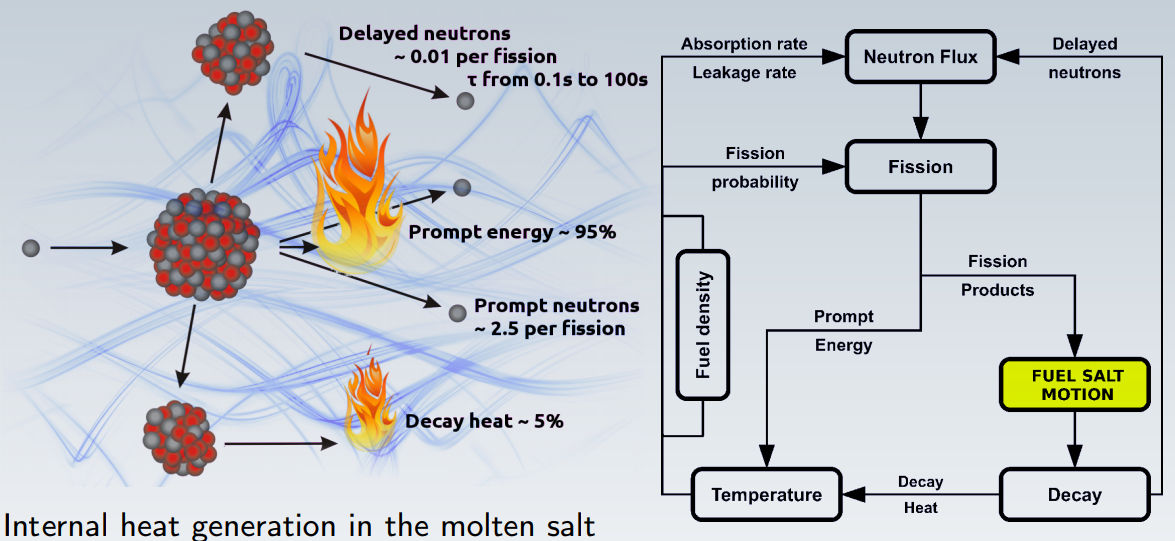
\includegraphics[height=0.47\textwidth]{./images/coupled_physics.png}
		\vspace*{-0.05in}
		\caption{Challenges in simulating \glspl{MSR} (Image courtesy of Manuele Aufiero,2012).}
     	 \end{figure}               
\end{frame}

\begin{frame}
  \frametitle{Research objectives}
                  \vspace*{-0.1in}

              \begin{block}{Multiphysics simulation of \gls{MSR} (Moltres/MOOSE)\cite{lindsay_introduction_2018}}
               \begin{enumerate}
                \item Demonstrate steady-state and transient coupling of neutron fluxes, precursor drift, and thermal-hydraulics
                \item Implement advective movement of delayed neutron precursors
                \item Demonstrate capabilities with 2D axisymmetric and 3D mesh
                \item Simple transients: change of flow and moderator movement
               \end{enumerate}
               \end{block}


              
\end{frame}

\section{Methodology}
\subsection{Basics}
\begin{frame}
        \frametitle{Acquiring Moltres}
             \texttt{git clone https://github.com/arfc/moltres}\\
        \texttt{cd moltres}\\
        \texttt{git submodule init}\\
        \texttt{git submodule update}\\
\end{frame}


\begin{frame}
  \frametitle{Moltres (coupling in MOOSE)}
   \begin{block}{Moltres principal concept \cite{lindsay_introduction_2018}}
     \begin{itemize}
        \item Moltres is built on top of the Multi-physics Object-Oriented
Simulation Environment (MOOSE)
		\item MOOSE interfaces with libMesh to discretize simulation volume
into finite elements
		\item Provides interface for coding residuals that correspond to weak
form of governing PDEs; also interface for coding Jacobians $\Rightarrow$
more accurate Jacobians $\Rightarrow$ more efficient convergence
		\item Residuals and Jacobians send to PetSc which handles solution of resulting non-linear system of algebraic equations
     \end{itemize}
    \end{block}
               \begin{figure}[t]
                \vspace*{-0.15in}
                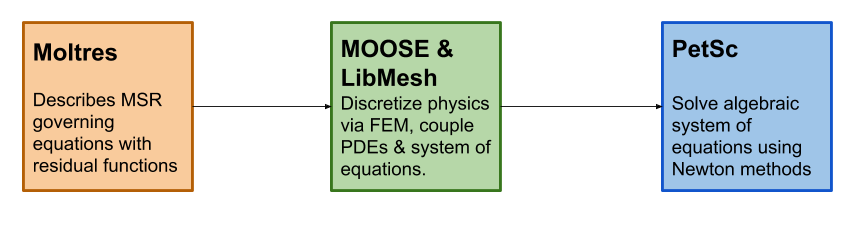
\includegraphics[height=0.24\textwidth]{./images/moltres-moose-diag.png}
                \vspace*{-0.1in}
                \caption{Moltres principal scheme}
               \end{figure}   
\end{frame}

\begin{frame}
	\frametitle{Intro to Moltres}
    	\begin{itemize}
			\item Liquid-fueled, molten salt reactors
			\item Multi-group diffusion (arbitrary number of groups)
			\item Advective movement of delayed neutron precursors
			\item Reynolds-averaged Navier-Stokes thermal hydraulics
			\item 2D axisymmetric
			\item 3D unstructured or structured
	    \end{itemize}
\end{frame}

\subsection{Kernels}
\begin{frame}
        \frametitle{Moltres Kernels}
        \footnotesize{Typical symbols (e.g. $\phi=\mbox{ neutron flux}$, 
                $T=\mbox{ temperature}$, and $C=\mbox{ precursor 
                concentrations}$).

\begin{align*}
\intertext{CoupledFissionEigenKernel} 
&\frac{\chi_g^p}{k} \sum_{g' = 1}^G (1 -
        \beta) \nu \Sigma_{g'}^f \phi_{g'}\\
\intertext{CoupledFissionKernel} 
&\chi_g^p \sum_{g' = 1}^G (1 -
        \beta) \nu \Sigma_{g'}^f \phi_{g'}\\
\intertext{CoupledScalarAdvection} 
&\nabla \cdot \vec{a} u\\
\intertext{DelayedNeutronSource} 
&\chi_g^d \sum_i^I \lambda_i C_i\\
\intertext{DivFreeCoupledScalarAdvection}
&\vec{a} \cdot \nabla u
\end{align*}}
\end{frame}

\begin{frame}
        \frametitle{Moltres Kernels}
        \footnotesize{
\begin{align*}
\intertext{FissionHeatSource}
&\frac{P}{\int_{\partial V} \sum_{g' = 1}^G \nu \Sigma_{g'}^f \phi_{g'} dV}
\sum_{g' = 1}^G \nu \Sigma_{g'}^f \phi_{g'}\\
\intertext{GammaHeatSource} &\gamma Q_f\\
        &\gamma = \mbox{moderator heat dissipation by gamma and neutron 
        irradiation}\\
        &Q_f = \sum_{g=1}^G \epsilon_{f,g}\Sigma_{f,g}\phi_g\\
        &\epsilon_{f,g} = \mbox{ heat per fission event.}\\
\intertext{GroupDiffusion}
& \nabla \cdot D_g
        \nabla \phi_g\\
\end{align*}
}
\end{frame}

\begin{frame}
        \frametitle{Moltres Kernels}
\footnotesize{
\begin{align*}
\intertext{InScatter}
&\sum_{g \ne g'}^G
        \Sigma_{g'\rightarrow g}^s \phi_{g'}\\
\intertext{NtTimeDerivative}
&\frac{1}{v_g}\frac{\partial \phi_g}{\partial t}\\
\intertext{PrecursorDecay}
&\lambda_i C_i\\
\intertext{PrecursorSource}
&\sum_{g'= 1}^G \beta_i \nu
        \Sigma_{g'}^f \phi_{g'}\\
\intertext{ScalarAdvectionArtDiff}
&\nabla \cdot -\delta \nabla u\\
        &\delta = \mbox{artificial diffusion coefficient}\\
        &\delta = \frac{|\vec{a}| h_{max}}{2}\\
        &\vec{a} = \mbox{advection velocity}\\
        &h_{max} = \mbox{max element length}
\end{align*}
}
\end{frame}

\begin{frame}
        \frametitle{Moltres Kernels}
        \footnotesize{
\begin{align*}
\intertext{ScalarTransportTimeDerivative}
&\frac{\partial u}{\partial t}\\
\intertext{SelfFissionEigenKernel}
&\frac{-\nu_f \Sigma_f \phi}{k}\\
\intertext{SigmaR}
&\Sigma_g^r \phi_g\\
\intertext{TransientFissionHeatSource}
&\sum_{g=1}^G \epsilon_{f,g}\Sigma_{f,g}\phi_g\\
\end{align*}
        }
\end{frame}


%\begin{frame}
%  \frametitle{Moltres Kernels}
%    \begin{columns}
%    \column[t]{6cm}
%               \begin{figure}[t]
%                  \vspace*{-0.15in}
%                 \hspace*{-0.35in}
%                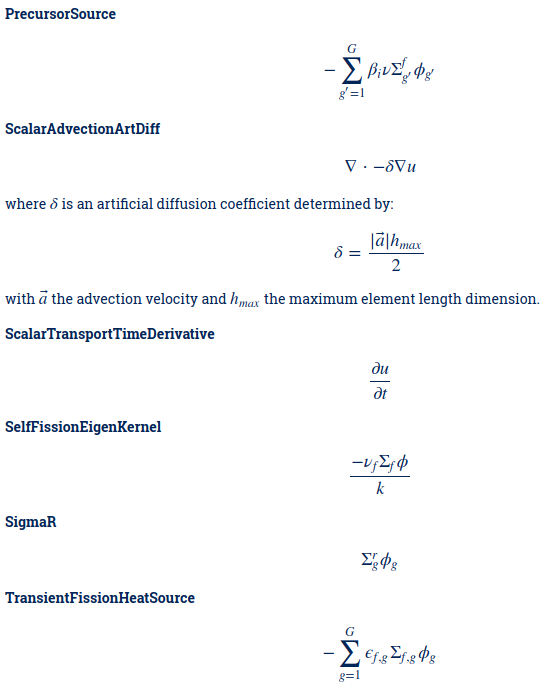
\includegraphics[height=1.15\textwidth]{./images/kernels4.png}
%               \end{figure}   
%
%    \column[t]{6cm}
%	\begin{itemize}
%		\item Kernels are individual pieces of governing equations
%		\item Modular (i.e. ``Diffusion" kernel could be used equally well to describe conduction or viscous shear)
%	\end{itemize}
%    \end{columns}  
%  
%\end{frame}
%
%\begin{frame}
%  \frametitle{Moltres Kernels (2)}
%               \begin{figure}[t]
%               \vspace*{-0.1in}
%                 \hspace*{-0.35in}
%                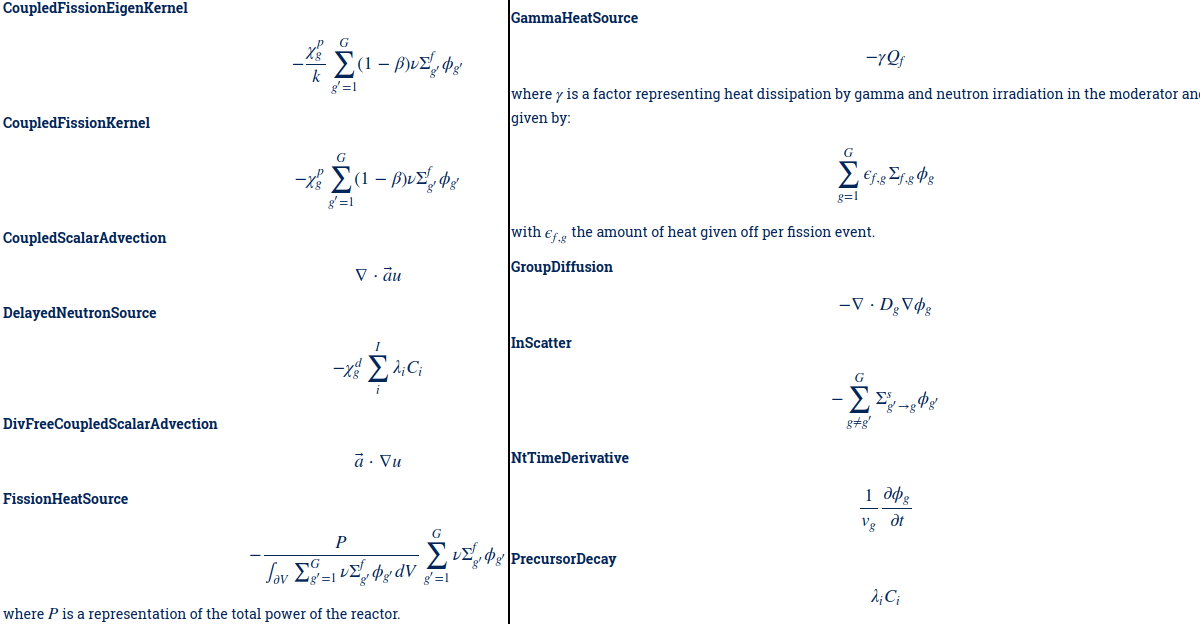
\includegraphics[height=0.6\textwidth]{./images/kernels11.png}
%               \end{figure}   
%\end{frame}

\subsection{Governing Equations}

\begin{frame}
  \frametitle{Governing Equations}
      \begin{block}{Time-dependent multi-group diffusion}
              \begin{figure}[t]
               \hspace*{-0.25in}
                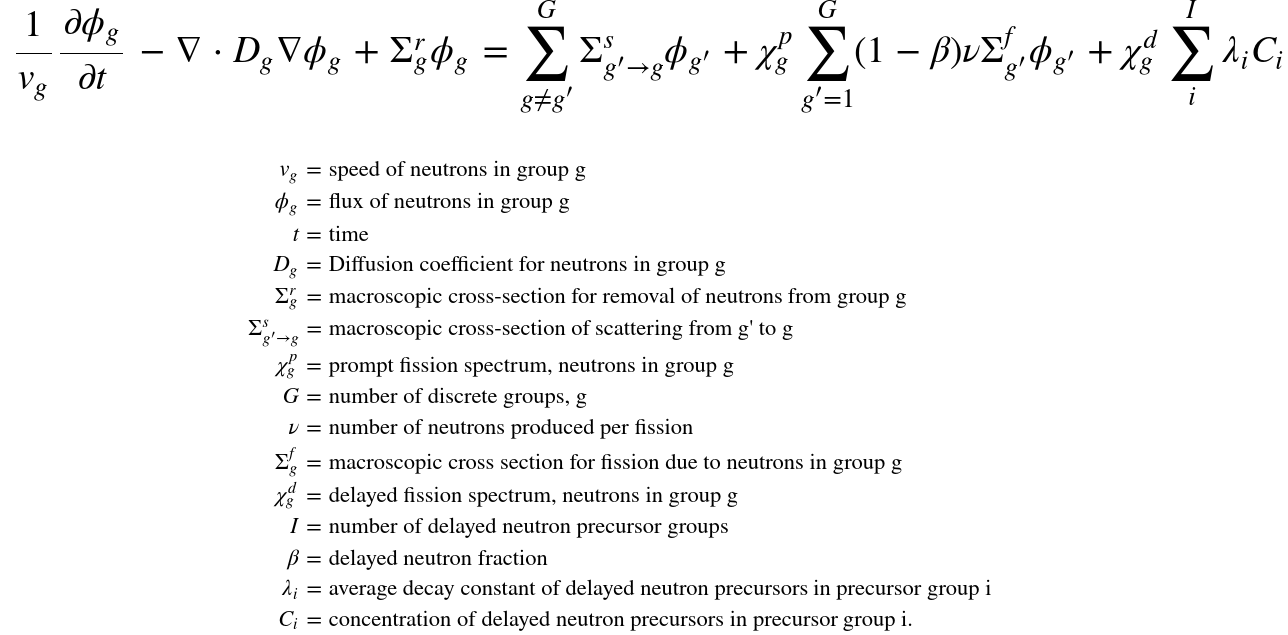
\includegraphics[height=0.55\textwidth]{./images/diffusion.png}
               \end{figure}   
      \end{block}
\end{frame}

\begin{frame}
  \frametitle{Governing Equations (2)}
     \begin{block}{Delayed neutron precursors}
               \begin{figure}[t]
                 \vspace*{-0.05in}
                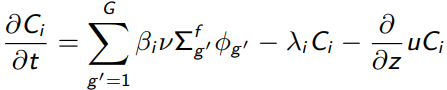
\includegraphics[height=0.07\textwidth]{./images/delayed_neutrons.png}
               \end{figure}   
     \end{block}
     
     \begin{block}{Heat conduction-convection with fission source in fuel}
              \begin{figure}[t]
                 \vspace*{-0.05in}
                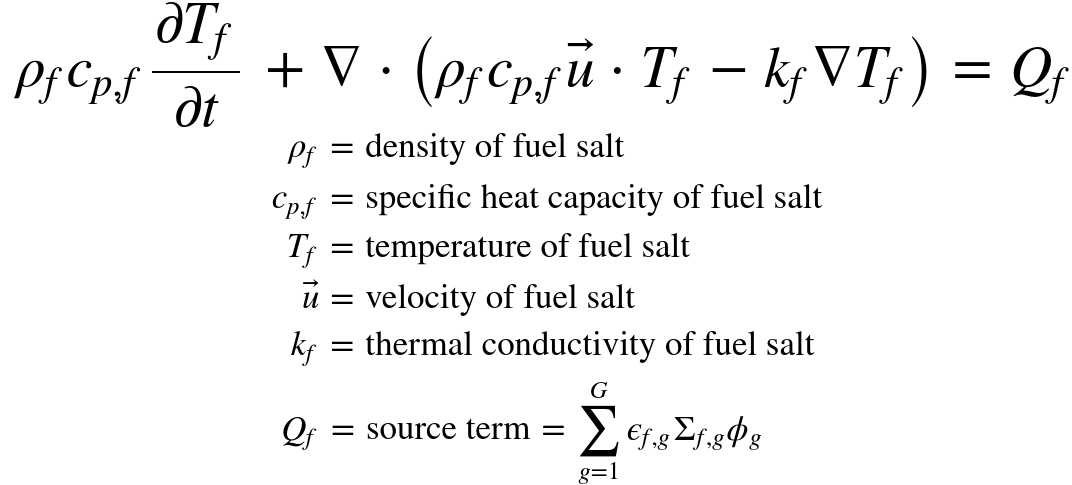
\includegraphics[height=0.21\textwidth]{./images/fuel_temp.png}
               \end{figure}        
	\end{block}
	
     \begin{block}{Heat conduction with option for irradiation source in moderator}
              \begin{figure}[t]
                 \vspace*{-0.05in}
                 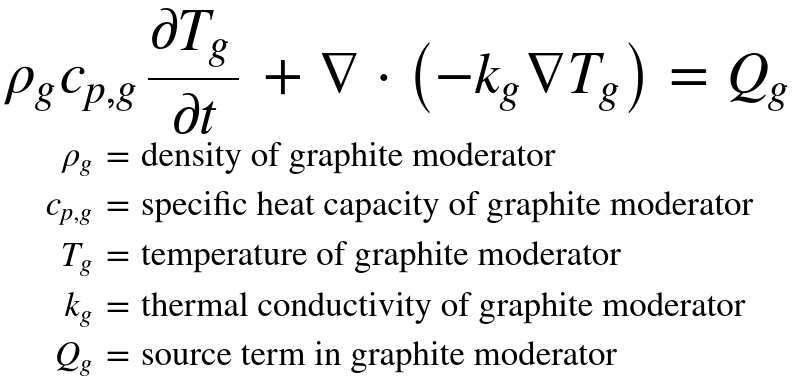
\includegraphics[height=0.17\textwidth]{./images/moder_temp.png}
               \end{figure}        
	\end{block}
\end{frame}

\begin{frame}
  \frametitle{Moltres \gls{MSRE} Simulations}
              \begin{figure}[t]
               \hspace*{-0.25in}
                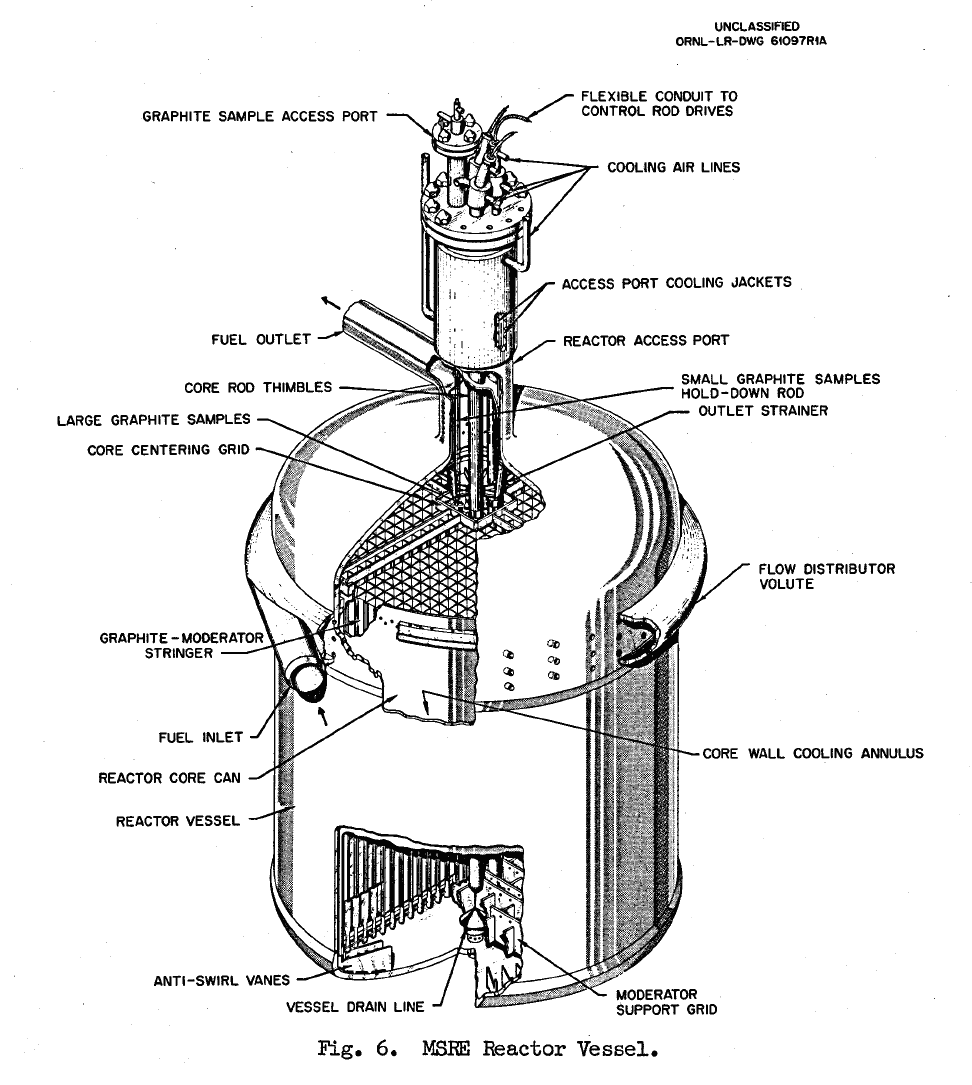
\includegraphics[height=0.65\textwidth]{./images/msre.png}
               \end{figure}   
\end{frame}

%\begin{frame}
%  \frametitle{Moltres MSRE Simulation: Input Data}
%     \begin{block}{Main input parameters \cite{lindsay_introduction_2018}}
%     	\begin{itemize}
%     		\item 22.5\% fuel volume fraction
%     		\item 2D axisymmetric and 3D core geometries derived 
%                        Group constants generated with SERPENT or NEWT (3D or 2D)
%     	\end{itemize}
%              \begin{figure}[t]
%                 \vspace*{-0.15in}
%                 \hspace*{-2.0in}
%                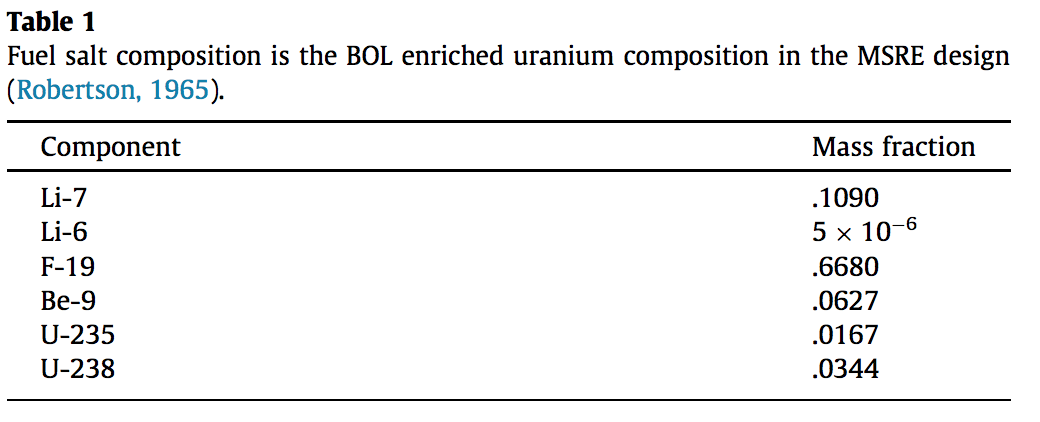
\includegraphics[height=0.2\textwidth]{./images/moltres-composition.png}
%               \end{figure}     
%               \begin{figure}[t]
%                 \vspace*{-0.25in}
%                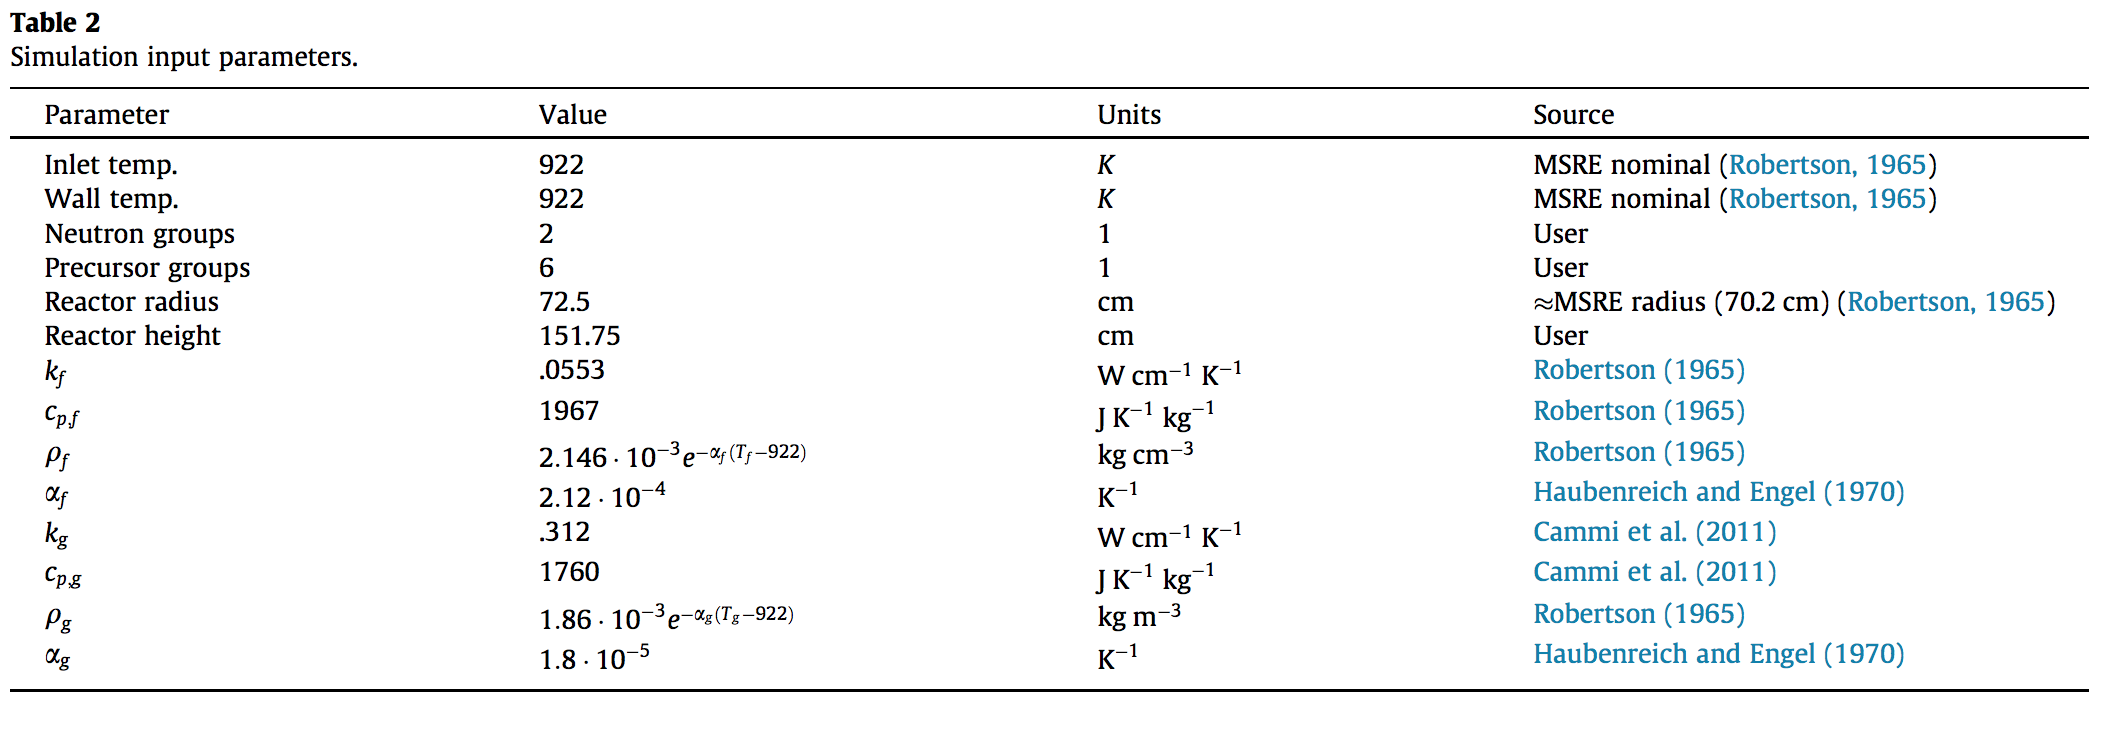
\includegraphics[height=0.33\textwidth]{./images/moltres-input.png}
%               \end{figure}   
%	\end{block}
%	
%\end{frame}

\section{Results}
\begin{frame}
  \frametitle{Multiphysics simulation results (2D)}
  \begin{figure}
   \vspace{-0.1in}
   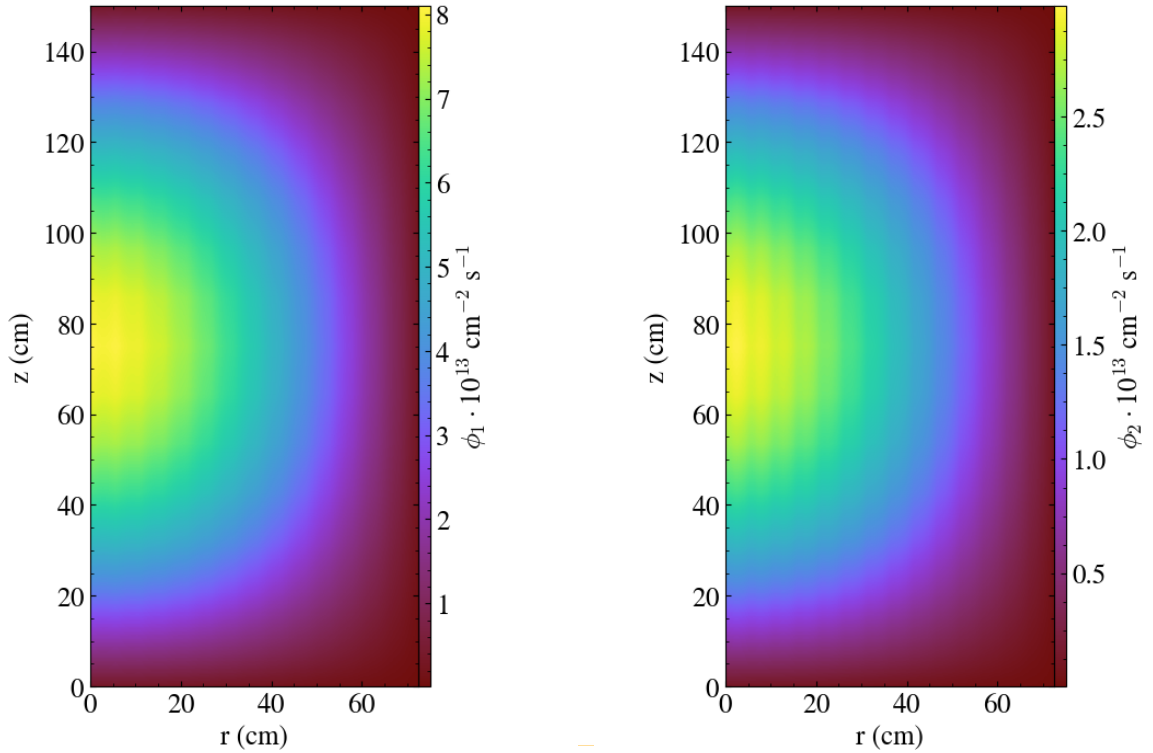
\includegraphics[height=0.85\textheight]{./images/moltres_flux.png}
   \vspace{-0.1in}
   \caption{Fast ($\phi_1$) and thermal ($\phi_2$) neutron flux obtained using Moltres 			\cite{lindsay_introduction_2018}.}
    \end{figure}
\end{frame}

\begin{frame}
  \frametitle{Multiphysics simulation results (2D) (2)}
  \begin{figure}[t]
   \vspace{-0.05in}
   \hspace*{-0.15in}
   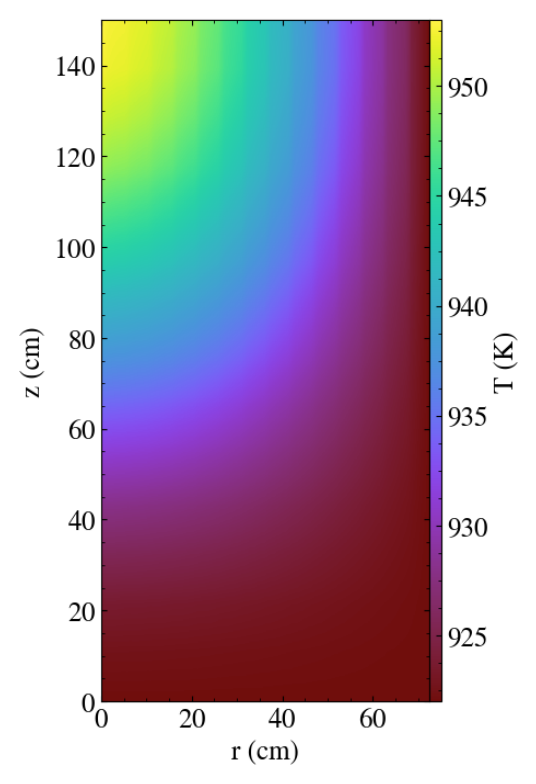
\includegraphics[height=0.85\textheight]{./images/moltres_temp.png}
   \vspace{-0.1in}
   \caption{Temperature in channel obtained using Moltres \cite{lindsay_introduction_2018}.}
    \end{figure}

\end{frame}

\begin{frame}
  \frametitle{Moltres vs MSRE Comparison}
  \begin{figure}[t]
   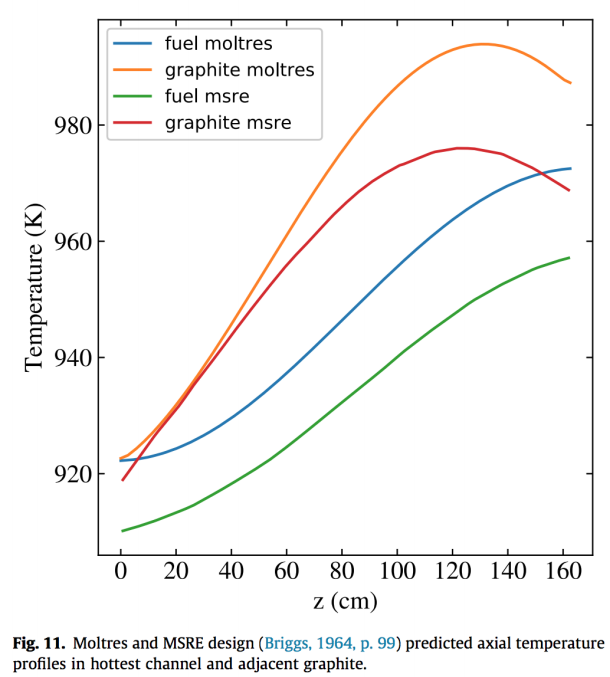
\includegraphics[height=0.85\textheight]{./images/msre_temp.png}
    \end{figure}

\end{frame}

\begin{frame}
  \frametitle{Moltres vs MSRE Comparison (2)}
  \begin{figure}[t]
   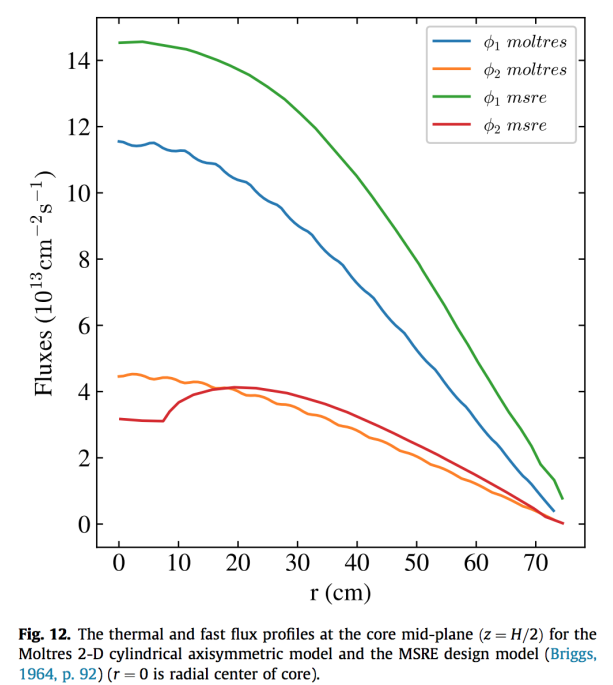
\includegraphics[height=0.85\textheight]{./images/msre_radial_flux.png}
    \end{figure}

\end{frame}

\begin{frame}
  \frametitle{Moltres vs MSRE Comparison (3)}
  \begin{figure}[t]
   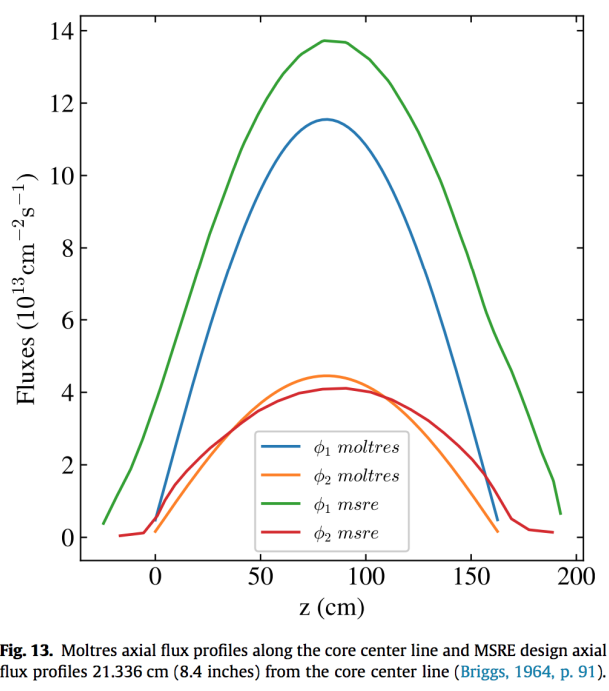
\includegraphics[height=0.85\textheight]{./images/msre_axial_flux.png}
    \end{figure}

\end{frame}

\begin{frame}
  \frametitle{Multiphysics simulation results (3D)}
  \begin{figure}[t]
   \vspace{-0.15in}
   \hspace*{-0.8in}
   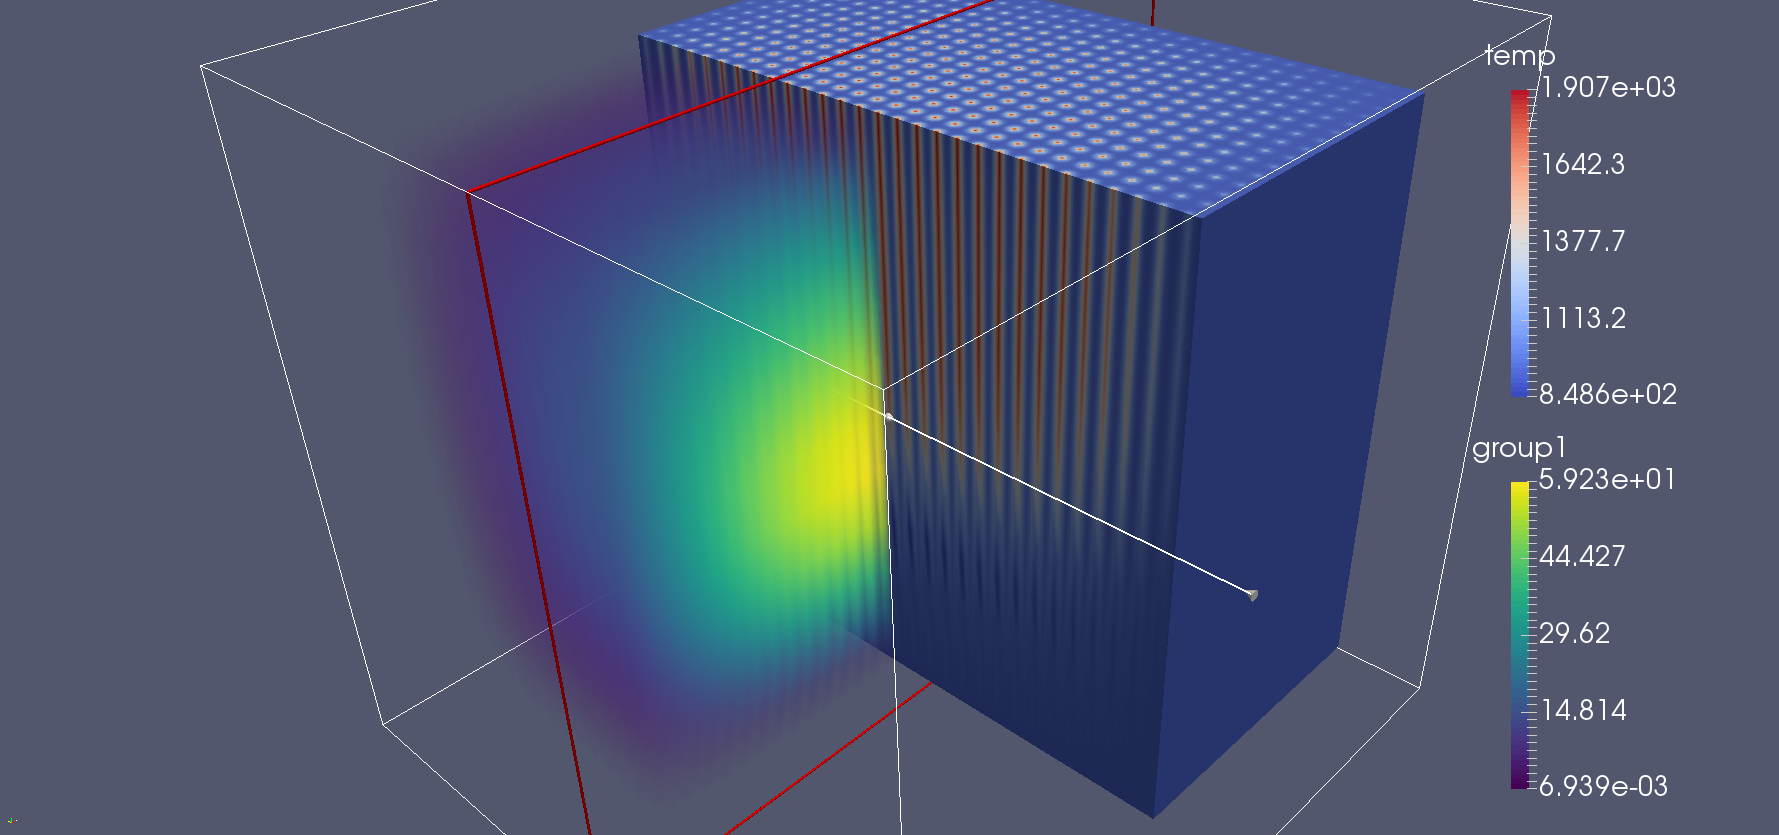
\includegraphics[height=0.8\textheight]{./images/moltres_3D.png}
   \caption{\gls{MSRE} steady-state temperature and fast neutron flux \cite{ridley_introduction_2017}.}
    \end{figure}
\end{frame}

%\begin{frame}
%\includemedia[
%  activate=pageopen,
%  width=540pt,height=400pt,
%  addresource=./videos/test.mp4,
%  flashvars={%
%     source=./videos/test.mp4% same path as in addresource!
%   &autoPlay=true%    % optional configuration
%   &loop=true%        % variables
%  }  
%]{}{APlayer.swf}
%\end{frame}
\section{Conclusions}
\begin{frame}
  \frametitle{Conclusions}
		\begin{block}{Moltres}
		\begin{itemize}
		\item New tool \textbf{Moltres} was developed for modeling coupled physics in novel molten salt reactors
		\item 2D-axisymmetric and 3D multiphysics models are presented
		\item \textbf{Moltres} demonstrated strong parallel scaling (up to 384 physical cores) but further optimization required
        \end{itemize}
        \end{block}
        
\end{frame}

\begin{frame}
  \frametitle{Future work}       
              \begin{block}{Future research effort}
               \begin{enumerate}
                \item Validation with other multiphysics codes for various \gls{MSR} designs
                \item Include two-phase flow capabilities (gaseous fission products appear in the liquid salt, hence, salt cannot be considered incompressible)
                \item Flow vortices and similar thermal hydraulic phenomena representation
                \item Add realistic natural circulation (better than Boussinesq approximation)
                \item Incorporate compressibility of fuel salt
                \item Implement higher fidelity methods for neutron transport 
                \item Realistic thermal hydraulic will enable more realistic precursor drift
               \end{enumerate}
               \end{block}
\end{frame}

\begin{frame}
  \frametitle{Future work}       
              \begin{block}{Improving Moltres TH capabilities with high fidelity Nek5000 CFD framework \cite{obabko_verification_2015}}
               \begin{enumerate}
                \item Investigate vortex formation with single channel and partial core models in Nek5000
                \item Based on results decide which method to use instead of Reynolds-averaged Navier-Stokes
                \item Generate Reduced Order Model based on produced data
                \item The model will be used to establish functional kernel forms for laminar-turbulent transitional flow behavior predictive of vortices in Moltres
               \end{enumerate}
               \end{block}
\end{frame}
\section{Acknowledgements}
\begin{frame}
  \frametitle{Acknowledgement}
  \begin{itemize}
    \item This research is part of the Blue Waters sustained-petascale computing project, 
which is supported by the National Science Foundation (awards OCI-0725070 and 
ACI-1238993) and the state of Illinois.
    \item Andrei Rykhlevskii is supported by the Department of Nuclear, Plasma, and Radiological Engineering.
    \item Kathryn Huff is additionally supported by the NRC Faculty Development Program, the NNSA (awards 
    DE-NA0002576 and DE-NA0002534), and the International Institute for Carbon Neutral Energy Research (WPI-I2CNER).
    \item The authors would like to thank  members of Advanced Reactors and Fuel Cycles
research group (ARFC) at the University of Illinois at Urbana Champaign who 
provided valuable code reviews and proofreading.
    \item Alex Lindsay (Idaho National Laboratory), Gavin Ridley (Yellowstone Energy), Alvin Lee, Tomasz Kozlowski (University of Illinois)
  \end{itemize}
    \begin{figure}[t]
   \hspace*{-0.4in}
   
\includegraphics[height=0.25\textheight]{./images/acks.png}
    \end{figure}
\end{frame}

%%--------------------------------%%
%%--------------------------------%%
\begin{frame}[allowframebreaks]
  \frametitle{References}
  \bibliographystyle{unsrt}
  {\footnotesize \bibliography{bibliography.bib} }

\end{frame}

%%--------------------------------%%
%%---BACKUP SLIDES----------------%%




\end{document}



